\documentclass[conference]{IEEEtran}
\usepackage{cite}
\usepackage{graphicx}
\usepackage{booktabs}
\usepackage{xcolor}
\usepackage{url}
\usepackage{amsmath}

% Marks a number that waits for experiments/paper_batch.sh. Remove before submission.
\newcommand{\pending}[1]{\textcolor{red}{[#1]}}

\begin{document}

\title{Ask Less, Tell More: Rule Granularity, Not Prediction,\\Explains the Gains of OpenFlow Rule Pre-Installation}

% TODO: author names, affiliation and e-mail as the venue requires (double-blind venues: remove).
\author{\IEEEauthorblockN{Author One, Author Two, Author Three}
\IEEEauthorblockA{Department of Computer Science and Information Systems\\
BITS Pilani, India}}

\maketitle

\begin{abstract}
A reactive OpenFlow controller makes the first packet of every new flow wait for a rule; a proactive one does not wait but installs rules for every host pair. Many strategies in between have been proposed (longer timeouts, caches of popular rules, hybrids and machine-learned predictors), and each was evaluated on its own traffic, usually against a reactive controller that installs one exact-match rule per flow. We compare these strategies side by side on one emulated testbed (Mininet, Open vSwitch, POX), on a campus tree, a data-centre fat-tree and the real Abilene backbone, under university, web-search, data-mining and real ISP traffic, with identical flows for every controller. Our main finding is that the baseline, not the strategy, explains most of the reported gains: a reactive controller that installs one rule per destination on the first miss, with no prediction, finds a rule for 93.6--99.6\% of new connections on networks of 11--16 hosts, matches proactive's flow completion times, and beats a budgeted popularity hybrid and even its hindsight oracle. A trace-replay model that reproduces the hit rate of all 46 measured wildcard runs (mean absolute error at most 0.1 percentage points) extends the comparison to 1,024 hosts and shows where prediction starts to matter: on networks of hundreds of hosts, where flows per host pair fall to 2--3, a frequency counter adds 5--10 points over the best coarse-rule controller. Finally, we separate the two jobs of a PACKET\_IN, asking for a rule and telling the controller a flow exists: a controller that forwards on destination rules and copies only TCP SYN, FIN and RST packets is as fast as proactive on three of four networks, learns of 46,641 of 46,641 connections, and is unaffected when the controller is frozen.
\end{abstract}

\begin{IEEEkeywords}
software-defined networking, OpenFlow, flow-rule installation, benchmarking, rule caching, prediction
\end{IEEEkeywords}

\section{Introduction}

An OpenFlow switch forwards a packet only if it matches a rule. A \emph{reactive} controller installs a rule when a flow's first packet reaches it as a PACKET\_IN; a \emph{proactive} controller installs rules before traffic arrives. Reactive installation keeps tables small and gives the controller per-flow control, at the cost of a setup delay on every new flow and a controller request per flow per switch~\cite{ethane,difane,devoflow}. Proactive installation removes both costs but needs a rule for every host pair.

A large body of work sits between the two: adaptive timeouts~\cite{smarttime,ahihta}, caches of popular rules~\cite{cacheflow}, proactive/reactive hybrids~\cite{pard,kim2022}, and predictors, increasingly machine-learned, that install rules before the flows that need them~\cite{batista2024,rouf2025}. Each was shown to beat a reactive baseline. But that baseline changes two things at once compared with the proposed strategy: \emph{when} a rule is installed, and \emph{how coarse} it is. The common reactive baseline, the learning switch of NOX and POX, installs an exact-match rule for each transport connection. Such a rule is almost never reused, because every new TCP connection has a new source port. A pre-installed rule that matches a host pair, in contrast, serves every later connection of that pair. A predictor compared with exact-match reactive therefore gets credit for coarseness as well as for prediction.

We ask how much of the gain remains when the baseline uses the same coarse rules, and where prediction has room at all. Our contributions:
\begin{enumerate}
\item \textbf{A benchmark} of rule-installation strategies along four axes (timing, granularity, path choice, selection of pre-installed pairs) with identical flow schedules for every controller, four workloads taken from published measurements and real traffic matrices, three network types, and two bounds for any predictor: a random choice and a hindsight oracle (Section~\ref{sec:design}).
\item \textbf{The granularity finding.} Reactive with pair or destination rules finds a rule for 86--100\% of new connections at 11--16 hosts with no prediction, and dominates a budgeted popularity hybrid and its oracle (Section~\ref{sec:granularity}). Long timeouts give no benefit for short-flow traffic.
\item \textbf{A validated scale model and the regime map.} A trace replay reproduces the hit rate of the 46 measured wildcard runs (mean absolute error at most 0.1 points); on fat-trees of up to 1,024 hosts it shows that prediction pays only at hundreds of hosts, where flows per host pair fall to 2--3 (Section~\ref{sec:scale}).
\item \textbf{Asking versus telling.} A controller that forwards on destination rules and receives copies of TCP SYN, FIN and RST packets keeps proactive's speed and reactive's per-connection visibility (Section~\ref{sec:tap}).
\end{enumerate}
Of the 11 pre-installation papers in our survey (Section~\ref{sec:related}), none reports a coarse-rule reactive baseline or an upper bound. All code, flow schedules and per-flow results are released.\footnote{TODO: repository URL (anonymised for review if required).}

\section{Background and related work}\label{sec:related}

\textbf{Setup cost.} Ethane~\cite{ethane} and DIFANE~\cite{difane} measured the delay of reactive setup; DevoFlow~\cite{devoflow} showed that per-flow control overloads switch control paths and argued for wildcard rules by default, giving up visibility of most flows. Controller benchmarks~\cite{tootoonchian} measure peak request rates under synthetic load. We measure setup cost under realistic traffic, and show that the choice DevoFlow made for scalability also removes most of the case for prediction.

\textbf{Caching, timeouts and hybrids.} CacheFlow~\cite{cacheflow} caches popular rules and reports high hit rates on Zipf traffic. SmartTime~\cite{smarttime} and AH-IHTA~\cite{ahihta} tune timeouts. PARD~\cite{pard} forwards on coarse proactive rules while the controller installs detailed rules in the background; Kim et al.~\cite{kim2022} choose per flow between proactive and reactive in simulation. None compares against the others, or against a coarse-rule reactive controller, on the same traffic.

\textbf{Prediction.} Our survey covers 11 papers that pre-install rules using a predictor and 14 that use learning or heuristics for eviction and timeouts. Of the 11, four compare only against plain reactive installation (e.g., an LSTM scheduler on POX that reports 51\% lower response time~\cite{batista2024}), four do not name their baseline in the material available to us, and the other three compare against their own earlier variants, against routing-based placements, or study the benefit without a baseline; for nine of the 11 only the abstract was accessible. None reports a coarse-rule baseline or an upper bound. Where a simple baseline is reported in the eviction literature, the learned method's margin is small: a DQN eviction policy beats LFU by about 8\%~\cite{rouf2025}. Analytical models of reactive signalling and table occupancy exist~\cite{metter2017}; we use the same idea of replaying arrivals through a timeout cache, and validate it against measurement.

\textbf{Monitoring.} Flow records (sFlow, IPFIX~\cite{ipfix}) report flows after the fact or by sampling. Everflow~\cite{everflow} matches TCP SYN, FIN and RST packets in data-centre switches and mirrors them to collectors for tracing; FlowSense~\cite{flowsense} infers utilisation from the controller's existing messages. Our tap controller (Section~\ref{sec:tap}) uses Everflow's match inside the OpenFlow control loop, so the copy reaches the controller as a PACKET\_IN when the connection starts. We do not claim the mechanism as new; we measure what it changes in the reactive/proactive trade-off.

\textbf{Paths.} Fat-trees need ECMP or flow scheduling to use their capacity~\cite{alfares,hedera}. These works do not consider how rules are installed; we measure both together.

\section{Benchmark design}\label{sec:design}

\textbf{Testbed.} Mininet 2.3.0~\cite{mininet}, Open vSwitch 3.7.1~\cite{ovs} with the kernel datapath, POX 0.7.0 and OpenFlow 1.0, on one laptop (Windows 11 with WSL2, 16 hardware threads). The controller runs on the same machine. ARP tables are static and IPv6 is disabled, so neither reaches the controller.

\textbf{Controllers.} Table~\ref{tab:controllers} lists the strategies. All topology-aware controllers share one implementation that exposes the four axes as options, so two controllers differ only in the axis being compared.

\begin{table}[t]
\caption{Controllers. Timeouts: idle 10\,s, hard 30\,s unless stated.}\label{tab:controllers}
\centering\footnotesize
\begin{tabular}{@{}p{2.3cm}p{5.6cm}@{}}
\toprule
Name & Behaviour \\
\midrule
Reactive (tree) & POX learning switch, exact-match rule per connection per switch, over a spanning tree \\
Reactive, long & the same, idle 60\,s / hard 300\,s \\
Reactive, exact & exact-match rules on shortest paths (topology known) \\
Reactive, pair & one rule per (source, destination) MAC pair on the first miss \\
Reactive, dest. & one rule per destination MAC on the first miss \\
Counter $B$\% & reactive exact, plus pair rules for the top $B$\% of pairs by a decaying activity score (decay 0.97/s, hysteresis 1.5) \\
Oracle $B$\% & pair rules for the $B$\% of pairs that carry the most flows in this run, installed before the first flow \\
Random $B$\% & pair rules for $B$\% random pairs, before the first flow \\
Proactive & one rule per host pair on its lowest-delay path (ECMP on fat-trees, hashed per pair) \\
Tap & destination rules for every host, plus 3 rules per host that copy TCP SYN, FIN, RST to the controller \\
\bottomrule
\end{tabular}
\end{table}

\textbf{Networks.} A two-level campus tree (16 hosts, 5 switches, 240 ordered pairs); a $k{=}4$ fat-tree (16 hosts, 20 switches) and a $k{=}6$ fat-tree (54 hosts, 45 switches, 2,862 pairs); and the Abilene backbone (11 cities, 14 links, the real 2.48\,Gbit/s Atlanta--Indianapolis link scaled accordingly, one-way delays of 1.33--11.03\,ms from fibre distance). Links run at 100\,Mbit/s.

\textbf{Workloads.} \emph{University}: flow sizes from Benson et al.'s university data centres~\cite{benson}, Weibull gaps per edge switch with 80\% between 4 and 40\,ms. \emph{Web search} and \emph{data mining}: the DCTCP~\cite{dctcp} and VL2~\cite{vl2} size distributions as used by pFabric~\cite{pfabric} and PIAS~\cite{pias}, Poisson arrivals at 30\% load (5\% at $k{=}6$). \emph{ISP}: one day of real Abilene traffic matrices~\cite{zhang2005} replayed in 30\,s, SURGE flow sizes~\cite{surge}. Host-pair popularity is Zipf with exponent 1, as assumed by CacheFlow~\cite{cacheflow}, with a uniform control; the ISP workload uses the real matrices. Each flow is a TCP connection that sends its bytes and waits for a one-byte reply.

\textbf{Fairness and statistics.} The flow schedule is computed from a seed before the run, so every controller receives exactly the same flows. All controllers of a scenario run for each seed in one batch. We report the mean of 5 seeds (3 at $k{=}6$) with the half-width of the 95\% confidence interval (Student's $t$).

\textbf{Metrics.} \emph{Hit rate}: share of new TCP connections whose SYN finds a rule at the sender's switch, counted by the controller. \emph{Small-flow FCT}: median completion time of flows under 100\,KB. Controller load: PACKET\_IN/s and controller CPU. \emph{Rules}: peak rules over all switches, read from the switches. \emph{Visibility}: share of connections the controller learns of.

\section{Results on the testbed}\label{sec:granularity}

\subsection{Exact-match reactive pays twice}
Under realistic traffic, exact-match reactive sends 10.5--12.9 PACKET\_INs per flow and its small flows are 2.2--28$\times$ slower than proactive's. On networks with loops part of this is path, not setup: the spanning tree switches off 4 of Abilene's 14 links, so 70\% of pairs take a longer path (mean delay stretch 1.58, up to 4.47). Running the same exact-match controller on shortest paths splits the small-flow median penalty on Abilene into about 41\,ms of path and 10\,ms of setup. Long timeouts (60\,s/300\,s) gave no fewer controller requests and no faster flows in any of four scenarios, with 2.2--3.0$\times$ the rules: an exact-match rule is not reused by a new connection however long it lives.

\subsection{Granularity explains the hybrid's gain}

\begin{table}[t]
\caption{Coarse reactive rules against the budgeted hybrid (25\% budget). Mean of 5 runs; FCT is the small-flow median with 95\% CI.}\label{tab:granularity}
\centering\footnotesize
\setlength{\tabcolsep}{3.5pt}
\begin{tabular}{@{}lrrrr@{}}
\toprule
Controller & Hit \% & FCT (ms) & PKT\_IN/s & Rules \\
\midrule
\multicolumn{5}{@{}l}{\emph{University tree, 16 hosts, Zipf pairs}} \\
Reactive, exact & 0 & 52.5$\pm$5.0 & 2,352 & 10,987 \\
Reactive, pair & 97.9 & 1.49$\pm$0.27 & 34 & 624 \\
Reactive, dest. & 99.6 & 1.47$\pm$0.22 & 8 & 80 \\
Counter 25\% & 60.6 & 12.0$\pm$3.5 & 903 & 5,084 \\
Oracle 25\% & 68.2 & 6.3$\pm$1.2 & 646 & 3,589 \\
Random 25\% & 23.9 & 35.1$\pm$6.0 & 1,781 & 8,574 \\
Proactive & -- & 1.49$\pm$0.27 & 0 & 624 \\
\midrule
\multicolumn{5}{@{}l}{\emph{Fat-tree $k{=}4$, web search, 16 hosts}} \\
Reactive, pair & 86.1 & 39.2$\pm$18.8 & 115 & 832 \\
Reactive, dest. & 93.6 & 31.6$\pm$4.3 & 69 & 280 \\
Counter 25\% & 65.7 & 42.6$\pm$6.3 & 186 & 1,566 \\
Oracle 25\% & 73.7 & 36.8$\pm$4.6 & 141 & 1,223 \\
Proactive (ECMP) & -- & 28.7$\pm$5.2 & 0 & 1,072 \\
\midrule
\multicolumn{5}{@{}l}{\emph{Abilene, real traffic matrices, 11 hosts}} \\
Reactive, exact & 0 & 56.5$\pm$2.7 & 444 & 5,319 \\
Reactive, pair & 96.5 & 46.1$\pm$1.5 & 15 & 380 \\
Reactive, dest. & 97.8 & 46.1$\pm$1.6 & 6 & 120 \\
Counter 25\% & 52.2 & 50.9$\pm$2.5 & 207 & 2,621 \\
Oracle 25\% & 59.2 & 49.9$\pm$3.0 & 168 & 2,419 \\
Proactive & -- & 46.0$\pm$1.5 & 0 & 386 \\
\bottomrule
\end{tabular}
\end{table}

Table~\ref{tab:granularity} adds coarse-rule reactive controllers to the comparison. Exact-match rows for the fat-tree are omitted because that batch was disturbed by the host sleeping; an earlier clean batch gave 59.3\,ms for exact-match reactive on shortest paths against 28.6\,ms for proactive ECMP.

\textbf{Coarse rules close the gap without prediction.} Pair and destination rules find a rule for 86--100\% of new connections. On the university tree and Abilene their small-flow median equals proactive's within the interval, and they need no more rules than proactive (destination rules: 80 and 120 against 624 and 386).

\textbf{The hybrid is dominated.} At a 25\% budget the counter, and even the oracle that knows the run's busiest pairs in advance, have lower hit rates, more PACKET\_INs and 1.5--8$\times$ more rules than plain pair rules. The hybrid's gain over exact-match reactive came from the coarseness of its pre-installed rules, which its exact-match fallback lacks. Pair selection still matters relative to chance (counter 52--66\% against random 19--25\%), but it is not where the benefit lies.

\textbf{Skew is not required.} With uniform pair popularity, pair rules still reach 98.0\% (6,093 flows over 240 pairs is about 25 flows per pair in 30\,s), while the counter falls to its budget share (24.8\%).

\section{Where prediction has room: scale}\label{sec:scale}

The coarse-rule result depends on each pair carrying many flows while its rule is alive. At 54 hosts this no longer holds: the hit rate of pair rules falls to 50.8$\pm$5.0\% and of destination rules to 59.3$\pm$2.4\% (3 runs, about 640 flows over 2,862 pairs). Here the counter at a 10\% budget only equals pair rules (51.1\%) with 1.9$\times$ their rules, and only the oracle is clearly better (77.8\%).

\textbf{A validated replay model.} To go beyond what the laptop can emulate we replay flow schedules through a timeout cache (idle 10\,s, hard 30\,s): a pair or destination rule is created on a miss at every switch of the path and refreshed by each packet of later flows. Replaying the stored schedules of all 46 measured pair- and destination-rule runs (four scenarios with 5 seeds, plus $k{=}6$ with 3) reproduces the measured hit rates with a mean absolute error per run of at most 0.1 percentage points in every scenario. We then generate web-search schedules with the same code for fat-trees with $k$ from 4 to 16 (16 to 1,024 hosts) at 5\% and 30\% load, 3 seeds each, and add a predictor that can actually be built: a frequency counter that pre-installs the busiest 10\% of pairs \emph{of the previous 30\,s window} (same pair popularity, new arrivals), with pair rules for everything else.

\begin{figure}[t]
\centering
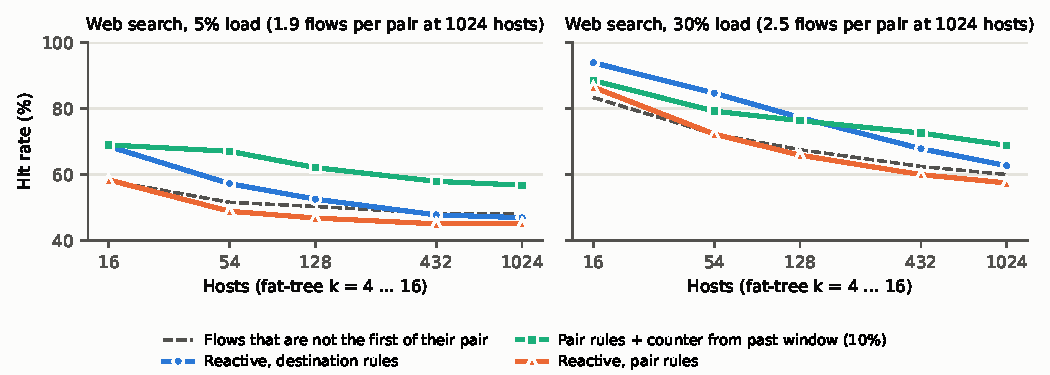
\includegraphics[width=\columnwidth]{scale_hit_rate.pdf}
\caption{Hit rate against network size (trace replay, mean of 3 seeds). The dashed line is the share of flows that are not the first of their host pair.}\label{fig:scale}
\end{figure}

Figure~\ref{fig:scale} shows the result.
\begin{itemize}
\item \textbf{Coarse rules lose hit rate as flows per pair fall.} At 30\% load, destination rules fall from 93.9\% at 16 hosts to 62.6\% at 1,024; flows per active pair fall from 6.0 to 2.5. Pair rules track the share of flows that are not the first of their pair: their misses are almost all first flows, which no reactive rule can serve.
\item \textbf{Prediction pays only in that regime.} At 16 hosts the history counter does not beat destination rules (88.5 vs.\ 93.9\% at 30\% load; 68.9 vs.\ 68.5\% at 5\%). At 30\% load it becomes the best non-hindsight strategy from 432 hosts (72.5 vs.\ 67.8\%; 68.8 vs.\ 62.6\% at 1,024). At 5\% load it beats destination rules by about 10 points from 54 hosts on.
\item \textbf{Hindsight bounds become uninformative at scale.} A 2--10\% budget of all pairs exceeds the number of pairs that appear in a 30\,s window at 432 hosts and more, so an oracle that knows the future reaches 100\%. Such bounds should be stated as a budget in rules, not as a share of pairs.
\end{itemize}

The practical boundary is set by table size, not only by hit rate. Proactive forwarding with destination rules needs exactly one rule per host per switch: 1,024 rules per switch at 1,024 hosts, within the range of hardware tables of DevoFlow's era~\cite{devoflow}. Prediction therefore earns its keep in networks with more hosts than a switch can hold destination rules for, and with few flows per pair, the case a predictor evaluation should target.

\section{Asking versus telling}\label{sec:tap}

A PACKET\_IN does two jobs: it \emph{asks} the controller where to send a packet, and it \emph{tells} the controller that a flow exists. Only asking delays the packet. Coarse rules and proactive installation remove the asking, but also the telling: with destination rules the controller hears of 0.4--6.4\% of connections on the small networks. Our tap controller keeps only the telling. Each switch has a destination rule per host, installed when it connects. At the switch a host is attached to, three higher-priority rules match TCP packets to that host with SYN (and not ACK), FIN or RST set; their actions forward the packet and send its first 128 bytes to the controller. No rule is installed per flow. TCP-flag matching is the Open vSwitch extension field \texttt{NXM\_NX\_TCP\_FLAGS}, sent from POX as a Nicira flow-mod; it is a standard match field in OpenFlow 1.5.

\begin{table}[t]
\caption{Tap against proactive and destination rules. Mean of 5 runs (3 at $k{=}6$); FCT is the small-flow median. Rules: peak total (busiest switch). ``Heard'' is the share of connections the controller learns of.}\label{tab:tap}
\centering\footnotesize
\setlength{\tabcolsep}{2.6pt}
\begin{tabular}{@{}lrrrr@{}}
\toprule
Controller & FCT (ms) & PKT\_IN/s & Rules & Heard \\
\midrule
\multicolumn{5}{@{}l}{\emph{University tree, 16 hosts}} \\
Reactive, exact & 35.7$\pm$5.7 & 2,486 & 11,392 (3,654) & 100\% \\
Reactive, dest. & 0.9$\pm$0.4 & 3 & 80 (16) & 0.4\% \\
Proactive & 0.9$\pm$0.4 & 0 & 624 (192) & 0\% \\
Tap & 1.0$\pm$0.4 & 602 & 128 (28) & 100\% \\
\midrule
\multicolumn{5}{@{}l}{\emph{Abilene, 11 hosts}} \\
Reactive, exact & 57.8$\pm$2.2 & 452 & 5,430 (855) & 100\% \\
Reactive, dest. & 46.1$\pm$1.6 & 5 & 121 (11) & 2.2\% \\
Proactive & 46.0$\pm$1.5 & 0 & 386 (62) & 0\% \\
Tap & 46.1$\pm$1.5 & 174 & 154 (14) & 100\% \\
\midrule
\multicolumn{5}{@{}l}{\emph{Fat-tree $k{=}6$, web search 5\%, 54 hosts}} \\
Reactive, exact & 51.9$\pm$8.4 & 362 & 2,341 (160) & 100\% \\
Reactive, dest. & 12.7$\pm$4.0 & 154 & 804 (26) & 40.7\% \\
Proactive (ECMP) & 5.0$\pm$0.7 & 0 & 13,230 (312) & 0\% \\
Tap & 5.3$\pm$1.1 & 63 & 2,592 (63) & 100\% \\
\midrule
\multicolumn{5}{@{}l}{\emph{Fat-tree $k{=}4$, web search 30\%, 16 hosts}} \\
Reactive, dest. & 31.7$\pm$4.6 & 60 & 285 (16) & 6.4\% \\
Proactive (ECMP) & 29.6$\pm$5.5 & 0 & 1,072 (58) & 0\% \\
Tap & 39.3$\pm$21.9 & 109 & 368 (22) & 100\% \\
\bottomrule
\end{tabular}
\end{table}

\textbf{Speed and visibility together.} Table~\ref{tab:tap} (a separate batch from Table~\ref{tab:granularity}, so absolute times differ slightly) shows that on the university tree, Abilene and the 54-host fat-tree, tap's small-flow median equals proactive's within the interval. The controller learned of all 46,641 connections in 21 runs. At 54 hosts, where coarse reactive rules miss often, tap's median is 2.4$\times$ lower than destination rules' and its controller receives 2.4$\times$ fewer messages, while hearing of every connection rather than 41\%.

\textbf{Rules.} Tap needs fewer rules than pair-rule proactive (128 vs.\ 624; 2,592 vs.\ 13,230 at 54 hosts), but this saving is granularity, not tapping: proactive with destination rules needs $H\cdot S$ rules for $H$ hosts and $S$ switches (80 and 2,430), and tapping adds exactly $3H$ (48 and 162).

\textbf{Cost.} About three copies per connection (602 PACKET\_IN/s and 14\% of one core at about 200 new connections per second on the university tree). None of them delays a packet.

\textbf{The $k{=}4$ fat-tree.} Here tap is slower than proactive ECMP (39.3 vs.\ 29.6\,ms) with a wide interval; one run had 3 failed flows of 1,111 and a 108\,ms mean, and large flows were slower in 4 of 5 runs. Tap spreads paths by destination, so all flows to one host share a path through the core, while proactive ECMP hashes per pair. Proactive with the same destination rules and paths, without the copies, gives \pending{X.X$\pm$X.X}\,ms, which \pending{does / does not} attribute the gap to path choice.

\textbf{A frozen controller.} We stop the POX process for 5\,s, 10\,s into the university workload (3 seeds, about 1,000 connections per run start in the window). Under exact-match reactive, 3,029 of 3,030 such connections took over 1\,s (small-flow median 5.0--6.0\,s, the TCP SYN retransmission times). Under destination rules, proactive and tap, 4 did, all in one seed under all three controllers; tap's median in the window was 1.3--2.0\,ms against 1.2--1.7\,ms for proactive. Only tap still accounted for every connection (18,269 of 18,269): the copies queue while the controller is stopped and are read when it resumes.

\section{Discussion}

\textbf{For evaluations of rule predictors.} Our results suggest three requirements. (1) Compare against reactive with the same rule granularity as the pre-installed rules; otherwise the measured gain mixes coarseness and prediction. (2) Report flows per active pair (or per rule key) for the evaluated traffic; it decides whether a coarse first-miss rule is reused, and therefore whether prediction can add anything. (3) State hindsight bounds with a budget in rules and alongside a realisable predictor; at scale a share-of-pairs oracle is trivially perfect.

\textbf{When each strategy wins.} On small networks, or wherever a switch can hold one rule per destination, proactive destination rules are fastest and smallest, and coarse reactive rules come close. Exact-match reactive is justified only by per-flow policy, which our workloads do not exercise. Prediction pays at large scale with few flows per pair. If the controller must know about each connection, tap provides that without the reactive wait, for TCP.

\textbf{Limitations.} The network is emulated in software, so there is no TCAM limit and no hardware rule-update rate; POX is single-threaded, so absolute controller numbers are POX's. The testbed networks have 11--54 hosts; larger sizes come from the replay model, which is validated for hit rate only, and its predictor is given stationary pair popularity, which favours prediction. Pair popularity is an assumed Zipf distribution except for the ISP workload, and the university size distribution was read from a published plot. Each run is 30\,s. Tap covers TCP only, records start and end but not bytes, and cannot take a decision before the first packet. The controller shares the host with the emulated network; we did not vary the control-channel delay. Results come from batches on different days with the same settings; absolute times are compared only within a table.

\section{Conclusion}
The gains reported for rule pre-installation and prediction are measured mostly against a reactive controller that installs one exact-match rule per connection. When the reactive baseline uses the same coarse rules as the pre-installed ones, it reaches 86--100\% hit rates on networks of up to 16 hosts and dominates a budgeted popularity hybrid and its oracle. Prediction becomes useful only when flows per host pair fall to 2--3, which in our model happens at hundreds of hosts. Separately, the visibility that reactive installation provides does not require making packets wait: copying connection start and end packets gives the controller every connection at proactive speed. We release the benchmark so that future predictors can be measured against these baselines.

\bibliographystyle{IEEEtran}
\begin{thebibliography}{99}
\bibitem{ethane} M. Casado, M.~J. Freedman, J. Pettit, J. Luo, N. McKeown, and S. Shenker, ``Ethane: Taking control of the enterprise,'' in \emph{Proc. ACM SIGCOMM}, 2007.
\bibitem{difane} M. Yu, J. Rexford, M.~J. Freedman, and J. Wang, ``Scalable flow-based networking with DIFANE,'' in \emph{Proc. ACM SIGCOMM}, 2010.
\bibitem{devoflow} A.~R. Curtis, J.~C. Mogul, J. Tourrilhes, P. Yalagandula, P. Sharma, and S. Banerjee, ``DevoFlow: Scaling flow management for high-performance networks,'' in \emph{Proc. ACM SIGCOMM}, 2011.
\bibitem{tootoonchian} A. Tootoonchian, S. Gorbunov, Y. Ganjali, M. Casado, and R. Sherwood, ``On controller performance in software-defined networks,'' in \emph{Proc. USENIX Hot-ICE}, 2012.
\bibitem{cacheflow} N. Katta, O. Alipourfard, J. Rexford, and D. Walker, ``CacheFlow: Dependency-aware rule-caching for software-defined networks,'' in \emph{Proc. ACM SOSR}, 2016.
\bibitem{smarttime} A. Vishnoi, R. Poddar, V. Mann, and S. Bhattacharya, ``Effective switch memory management in OpenFlow networks,'' in \emph{Proc. ACM DEBS}, 2014.
\bibitem{ahihta} B. Isyaku, K. Abu Bakar, M.~S. Mohd Zahid, and M.~N. Yusuf, ``Adaptive and hybrid idle--hard timeout allocation and flow eviction mechanism considering traffic characteristics,'' \emph{Electronics}, 2020.
\bibitem{pard} R. Rzepka, P. Boryło, A. Lasoń, and A. Szymański, ``PARD: Hybrid proactive and reactive method eliminating flow setup latency in SDN,'' \emph{J. Netw. Syst. Manag.}, vol.~28, 2020.
\bibitem{kim2022} Kim \emph{et al.}, ``Mobility-aware hybrid flow rule cache scheme in software-defined access networks,'' \emph{Electronics}, 2022. % TODO: check author list and exact title
\bibitem{batista2024} Batista \emph{et al.}, ``A new intelligent scheduler to improve reactive OpenFlow communication in SDN-based IoT data streams,'' \emph{Discover Internet of Things}, vol.~4, no.~15, 2024.
\bibitem{rouf2025} R. Rouf and M. Yuksel, ``Spatial encoding of flow spaces for flow table eviction,'' arXiv, 2025. % TODO: check exact title
\bibitem{metter2017} C. Metter, M. Seufert, F. Wamser, T. Zinner, and P. Tran-Gia, ``Analytical model for SDN signaling traffic and flow table occupancy and its application for various types of traffic,'' \emph{IEEE Trans. Netw. Serv. Manag.}, vol.~14, no.~3, 2017.
\bibitem{ipfix} B. Claise, B. Trammell, and P. Aitken, ``Specification of the IP Flow Information Export (IPFIX) protocol,'' RFC 7011, 2013.
\bibitem{everflow} Y. Zhu \emph{et al.}, ``Packet-level telemetry in large datacenter networks,'' in \emph{Proc. ACM SIGCOMM}, 2015.
\bibitem{flowsense} C. Yu, C. Lumezanu, Y. Zhang, V. Singh, G. Jiang, and H.~V. Madhyastha, ``FlowSense: Monitoring network utilization with zero measurement cost,'' in \emph{Proc. PAM}, 2013.
\bibitem{alfares} M. Al-Fares, A. Loukissas, and A. Vahdat, ``A scalable, commodity data center network architecture,'' in \emph{Proc. ACM SIGCOMM}, 2008.
\bibitem{hedera} M. Al-Fares, S. Radhakrishnan, B. Raghavan, N. Huang, and A. Vahdat, ``Hedera: Dynamic flow scheduling for data center networks,'' in \emph{Proc. USENIX NSDI}, 2010.
\bibitem{mininet} B. Lantz, B. Heller, and N. McKeown, ``A network in a laptop: Rapid prototyping for software-defined networks,'' in \emph{Proc. ACM HotNets}, 2010.
\bibitem{ovs} B. Pfaff \emph{et al.}, ``The design and implementation of Open vSwitch,'' in \emph{Proc. USENIX NSDI}, 2015.
\bibitem{benson} T. Benson, A. Akella, and D.~A. Maltz, ``Network traffic characteristics of data centers in the wild,'' in \emph{Proc. ACM IMC}, 2010.
\bibitem{dctcp} M. Alizadeh \emph{et al.}, ``Data center TCP (DCTCP),'' in \emph{Proc. ACM SIGCOMM}, 2010.
\bibitem{vl2} A. Greenberg \emph{et al.}, ``VL2: A scalable and flexible data center network,'' in \emph{Proc. ACM SIGCOMM}, 2009.
\bibitem{pfabric} M. Alizadeh \emph{et al.}, ``pFabric: Minimal near-optimal datacenter transport,'' in \emph{Proc. ACM SIGCOMM}, 2013.
\bibitem{pias} W. Bai, L. Chen, K. Chen, D. Han, C. Tian, and H. Wang, ``Information-agnostic flow scheduling for commodity data centers,'' in \emph{Proc. USENIX NSDI}, 2015.
\bibitem{zhang2005} Y. Zhang, Z. Ge, A. Greenberg, and M. Roughan, ``Network anomography,'' in \emph{Proc. ACM IMC}, 2005.
\bibitem{surge} P. Barford and M. Crovella, ``Generating representative web workloads for network and server performance evaluation,'' in \emph{Proc. ACM SIGMETRICS}, 1998.
\end{thebibliography}

\end{document}
